\newpage
\section{Motos patinetes electricos}
\label{anexo_motos_patinetes_electricos}

Una vez analizados diversos vehículos factibles para el reparto de comida a domicilio, se ha decidido indagar una alternativa a usar un único vehículo.

En el \autoref{anexo_scooter_electrico} y en el \autoref{anexo_patienete eléctrico} se ha debatido la mejor opción dentro de la gama de motocicletas eléctricas y patinetes eléctricos, respectivamente. En consecuencia, se plantea una alternativa eficiente y coherente que cohesiona a la perfección la autonomía que proporciona el modelo Askoll eS1, con el precio competitivo de las Infiniton CITYJam Pro.

Tomando en consideración que el reparto de los pedidos es homogéneo en todas las franjas horarias, el radio de alcance máximo es de 6 \glssymbol{km}, y la longitud de los pedidos contando ida y vuelta de media oscila entre los 5 y los 7,5 \glssymbol{km}; se puede suponer que la longitud de los recorridos también posee cierta uniformidad. Por ello, se estima que el número de pedidos que se han de repartir en un radio de 4 a 6 km desde el establecimiento, supondrá a lo sumo un 33 (por ciento) de los mismos.

La solución que se plantea es que las motocicletas eléctricas cubran ese porcentaje de pedidos lejanos en todos y cada uno de los tramos horarios estudiados, mientras que los pedidos de corto alcance se realicen en patinetes. De este modo, eliminamos el problema que presentaban los patinetes al no poder alcanzar todas las áreas donde se debían realizar las entregas, al mismo tiempo que se mejora el tiempo de entrega en pedidos cortos porque los patinetes no necesitan ser estacionados, pueden acompañar a su conductor hasta la misma puerta del cliente.

Una motocicleta eléctrica del modelo Askoll eS1 es capaz de realizar unos 100 km a carga completa, lo que equivale a 20 pedidos, suponiendo que los repartos tienen una duración media de 5 km, o 13 pedidos si se suponen 7,5 \glssymbol{km}. Realizando los mismos cálculos que en el \autoref{anexo_calculos_sobre_vehiculos}, pero reduciendo el número de pedidos a realizar en cada tramo horario, se obtiene que son necesarias unos 16 patinetes para la primera hipótesis contemplada (repartos individuales de 5 km) y 14 patinetes para el caso de realizar repartos dobles de 7,5 \glssymbol{km} de ida y vuelta, según la \autoref{tab: analisis_detallado_patinete_5km_2} y la \autoref{tab: analisis_detallado_patinete_7,5km_2}.

\begin{table}[H]
\centering
\begin{tabular}{l|c|c|c|c|}
\cline{2-5}
 & \begin{tabular}[c]{@{}c@{}}TRAMO \\ HORARIO 1\end{tabular} & \begin{tabular}[c]{@{}c@{}}TRAMO \\ HORARIO 2\end{tabular} & \begin{tabular}[c]{@{}c@{}}TRAMO \\ HORARIO 3\end{tabular} & \begin{tabular}[c]{@{}c@{}}TRAMO \\ HORARIO 4\end{tabular} \\ \cline{2-5} 
 & \begin{tabular}[c]{@{}c@{}}Lunes-Jueves \\ (9:00-20:00)\end{tabular} & \begin{tabular}[c]{@{}c@{}}Lunes-Jueves \\ (20:00-0:00)\end{tabular} & \begin{tabular}[c]{@{}c@{}}Viernes-Domingo \\ (9:00-20:00)\end{tabular} & \begin{tabular}[c]{@{}c@{}}Viernes-Domingo \\ (20:00-1:00)\end{tabular} \\ \hline
\multicolumn{1}{|l|}{Nº pedidos} & 30 & 40 & 44 & 90 \\ \hline
\multicolumn{1}{|l|}{\begin{tabular}[c]{@{}l@{}}Distancia total a \\ recorrer \glssymbol{km}\end{tabular}} & 150 & 200 & 220 & 450 \\ \hline
\multicolumn{1}{|l|}{\begin{tabular}[c]{@{}l@{}}Tiempo total de \\ reparto \glssymbol{minuto} \end{tabular}} & 660 & 240 & 660 & 300 \\ \hline
\multicolumn{1}{|l|}{\begin{tabular}[c]{@{}l@{}}Tiempo estimado \\ por pedido (\glssymbol{minuto}/pedido)\end{tabular}} & 20 & 20 & 20 & 20 \\ \hline
\multicolumn{1}{|l|}{\begin{tabular}[c]{@{}l@{}}Nº pedidos realizables \\ por vehículo\end{tabular}} & 33 & 12 & 33 & 15 \\ \hline
\multicolumn{1}{|l|}{\begin{tabular}[c]{@{}l@{}}Nº vehículos simultáneos \\ necesarios\end{tabular}} & 1 & 4 & 2 & 6 \\ \hline
\multicolumn{1}{|l|}{Nº de turnos de vehículos} & 4 & 8 & 3 & 2 \\ \hline
\multicolumn{1}{|l|}{\begin{tabular}[c]{@{}l@{}}Nº vehículos totales \\ necesarios\end{tabular}} & 4 & 8 & 6 & 12 \\ \hline
\end{tabular}
\caption{Análisis detallado del reparto en patinete con viajes de 5 \glssymbol{km}.}
\label{tab: analisis_detallado_patinete_5km_2}
\end{table}



\begin{table}[H]
\centering
\begin{tabular}{l|c|c|c|c|}
\cline{2-5}
 & \begin{tabular}[c]{@{}c@{}}TRAMO \\ HORARIO 1\end{tabular} & \begin{tabular}[c]{@{}c@{}}TRAMO \\ HORARIO 2\end{tabular} & \begin{tabular}[c]{@{}c@{}}TRAMO \\ HORARIO 3\end{tabular} & \begin{tabular}[c]{@{}c@{}}TRAMO \\ HORARIO 4\end{tabular} \\ \cline{2-5} 
 & \begin{tabular}[c]{@{}c@{}}Lunes-Jueves \\ (9:00-20:00)\end{tabular} & \begin{tabular}[c]{@{}c@{}}Lunes-Jueves \\ (20:00-0:00)\end{tabular} & \begin{tabular}[c]{@{}c@{}}Viernes-Domingo \\ (9:00-20:00)\end{tabular} & \begin{tabular}[c]{@{}c@{}}Viernes-Domingo \\ (20:00-1:00)\end{tabular} \\ \hline
\multicolumn{1}{|l|}{Nº pedidos dobles} & 7 & 12 & 17 & 47 \\ \hline
\multicolumn{1}{|l|}{\begin{tabular}[c]{@{}l@{}}Distancia total a \\ recorrer (\glssymbol{km})\end{tabular}} & 52,5 & 90 & 127,5 & 352,5 \\ \hline
\multicolumn{1}{|l|}{\begin{tabular}[c]{@{}l@{}}Tiempo total de \\ reparto doble (\glssymbol{minuto})\end{tabular}} & 660 & 240 & 660 & 300 \\ \hline
\multicolumn{1}{|l|}{\begin{tabular}[c]{@{}l@{}}Tiempo estimado por \\ pedido doble (\glssymbol{minuto}/pedido)\end{tabular}} & 32,5 & 32,5 & 32,5 & 32,5 \\ \hline
\multicolumn{1}{|l|}{\begin{tabular}[c]{@{}l@{}}Nº pedidos dobles \\ realizables por vehículo\end{tabular}} & 20 & 7 & 20 & 9 \\ \hline
\multicolumn{1}{|l|}{\begin{tabular}[c]{@{}l@{}}Nº vehículos simultáneos \\ necesarios\end{tabular}} & 1 & 2 & 1 & 6 \\ \hline
\multicolumn{1}{|l|}{Nº de turnos de vehículos} & 2 & 2 & 4 & 2 \\ \hline
\multicolumn{1}{|l|}{\begin{tabular}[c]{@{}l@{}}Nº vehículos totales \\ necesarios\end{tabular}} & 2 & 4 & 4 & 12 \\ \hline
\end{tabular}
\caption{Análisis detallado del reparto en patinete con viajes de 7,5 \glssymbol{km}.}
\label{tab: analisis_detallado_patinete_7,5km_2}
\end{table}

En la \autoref{fig:patinetes_caso1_2} se comprueba que, efectivamente, 2 de los 6 patinetes empleados en el turno de mañana son reutilizables para el turno de tarde, por lo que como máximo son necesarios 16 patinetes.
\begin{figure}[H]
    \centering
    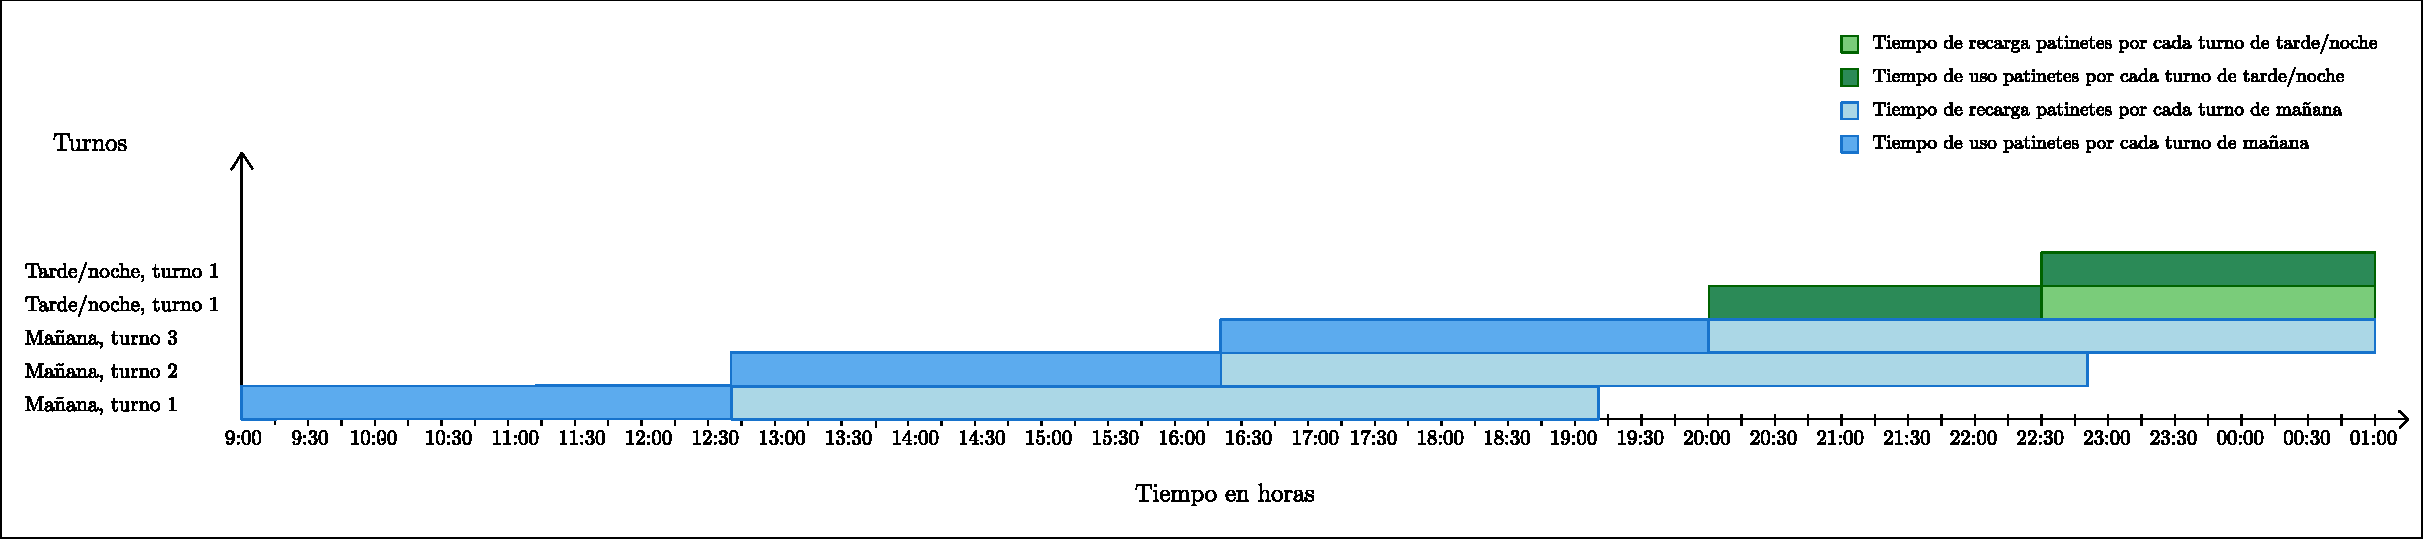
\includegraphics[width= \textwidth, height=12em]{archivos/caso2_patinetes.pdf}
    \caption{Representación turnos minorados de patinetes en viajes de 5 \glssymbol{km}.}
    \label{fig:patinetes_caso1_2}
\end{figure}

Igualmente, en la \autoref{fig:patinetes_caso2_2} se observa que uno de los patinetes se puede recargar y utilizar en el horario posterior, por lo que para esa hipótesis solo son necesarios 14 patinetes.

\begin{figure}[H]
    \centering
    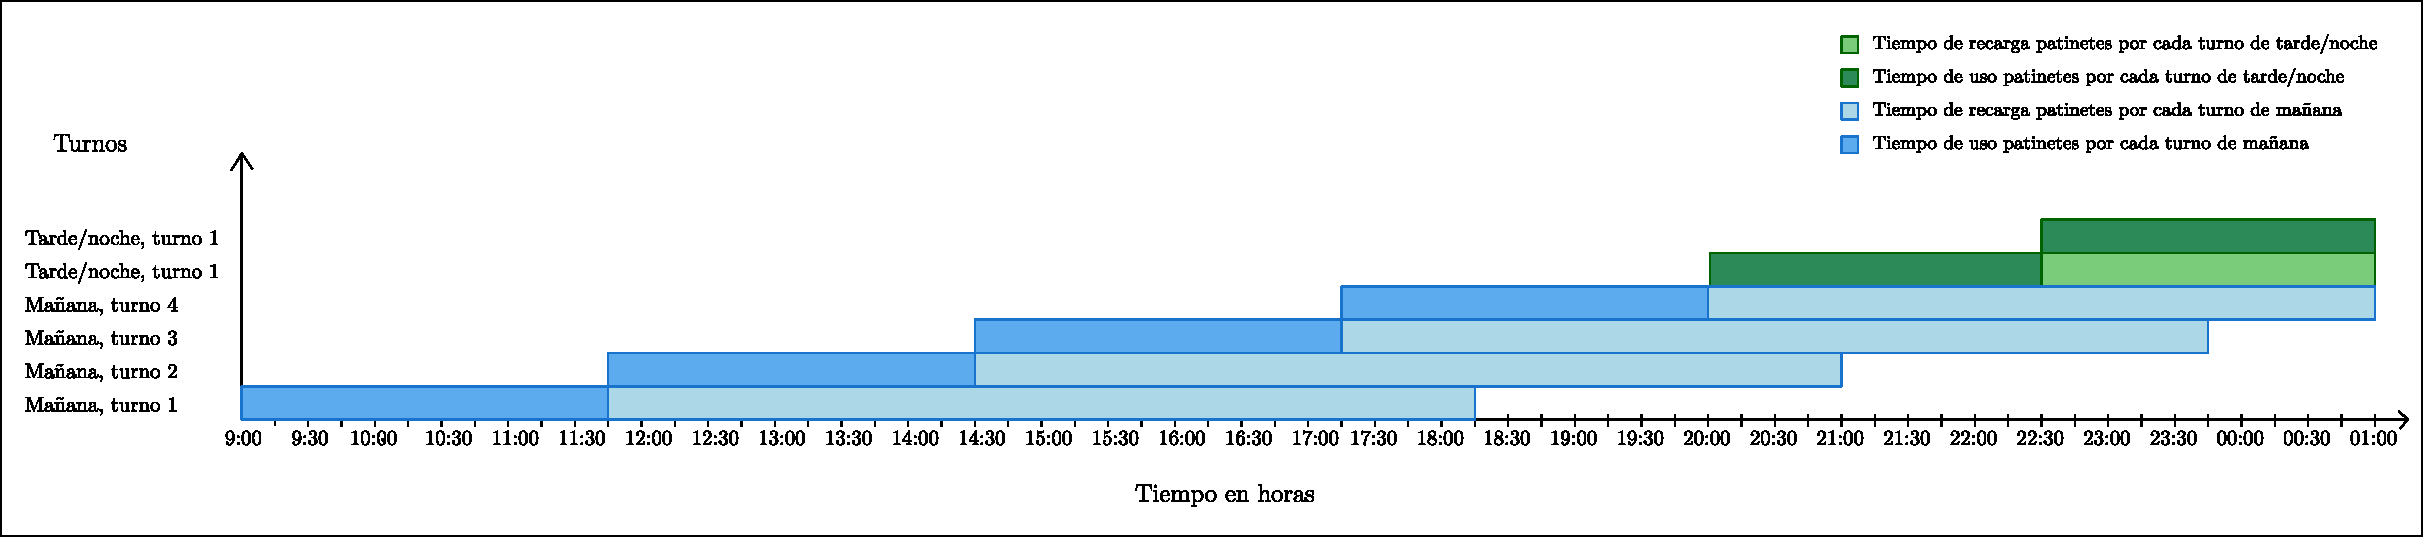
\includegraphics[width= \textwidth, height=12em]{archivos/caso1_patinetes.pdf}
    \caption{Representación turnos minorados de patinetes en viajes de 7,5 \glssymbol{km}.}
    \label{fig:patinetes_caso2_2}
\end{figure}

Finalmente, para hallar el presupuesto de esta opción híbrida se deben tener en cuenta diversos factores. 

Como se ha mencionado anteriormente, se supone  que las motocicletas cubren el 33 (por ciento) de los repartos, por ello los días entre semana se empleará una motocicleta para todo el día, mientras que en los fines de semana se usará una motocicleta en el turno de mañana y en el turno de tarde se ha de emplear la motocicleta del turno anterior además de otra a plena carga.

Respecto a los cálculos se ha de sumar el número de patinetes y sus costes asociados, así como los dos patinetes y sus respectivos costes, todo queda recogido en la \autoref{tab: analisis_presupuestos_patinetes_y_motos}. En estos cálculos se han empleado datos de la \autoref{tabla:tabla_datos_comunes}, de la \autoref{tab: analisis_presupuestos_patienetes} y de la \autoref{tab:Estudio presupuestos modelo Askoll eS1} debido a que estos modelos ya se han analizado en detalle en el \autoref{anexo_calculos_sobre_vehiculos}.

\begin{table}[H]
\centering
\begin{tabular}{|l|c|}
\hline
Nº recargas semanales patinetes caso 1 & 102 \\ \hline
Nº recargas semanales patinetes caso 2 & 72 \\ \hline
Nº recargas semanales motocicletas caso 1 & 10 \\ \hline
Nº recargas semanales motocicletas caso 2 & 10 \\ \hline
Presupuesto anual en recargas caso 1 (\glssymbol{euro}) & 330,01 \\ \hline
Presupuesto anual en recargas caso 2 (\glssymbol{euro}) & 268,90 \\ \hline
Presupuesto para vehículos primer año caso 1 (\glssymbol{euro}) & 16.536,67 \\ \hline
Presupuesto para vehículos primer año   caso 2 (\glssymbol{euro}) & 15.362,72 \\ \hline
Presupuesto para vehículos anual  caso 1 (\glssymbol{euro}) & 4.205,91 \\ \hline
Presupuesto para vehículos anual caso 2 (\glssymbol{euro}) & 3.785,20 \\ \hline
Presupuesto en vehículos a 10 años, caso 1 (\glssymbol{euro}) & 54.389,9 \\ \hline
Presupuesto en vehículos a 10 años, caso 2 (\glssymbol{euro}) & 49.429,53 \\ \hline
\end{tabular}
\caption{Análisis de los presupuestos opción óptima.}
\label{tab: analisis_presupuestos_patinetes_y_motos}
\end{table}


